\begin{figure}[ht!]
    \begin{subfigure}{\columnwidth}
    \centering
    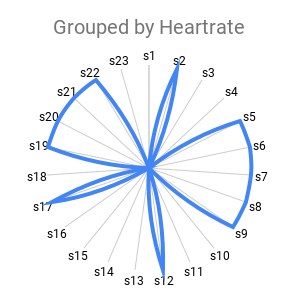
\includegraphics[width=.86\columnwidth]{figs/images/GroupedbyHeartrate.png}
    \caption{}
    \label{fig:g1}
    \end{subfigure}%
    \begin{subfigure}{\columnwidth}
    \centering
    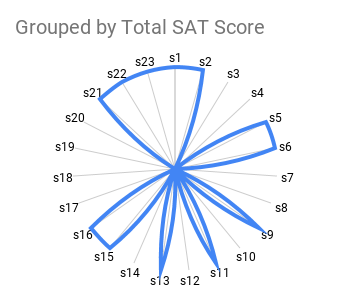
\includegraphics[width=\columnwidth]{figs/images/GroupedbyTotalSAT.png}
    \caption{}
    \label{fig:g2}
    \end{subfigure}
    
    \begin{subfigure}{\columnwidth}
    \centering
    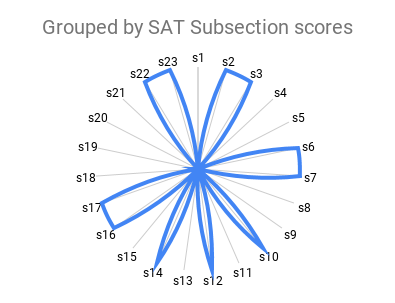
\includegraphics[width=1.13\columnwidth]{figs/images/GroupedbySATSubsection.png}
    \caption{}
    \label{fig:g3}
    \end{subfigure}%
    \begin{subfigure}{\columnwidth}
    \centering
    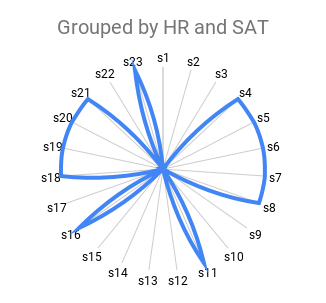
\includegraphics[width=.95\columnwidth]{figs/images/GroupedbyHRandSATSubsection.png}
    \caption{}
    \label{fig:g4}
    \end{subfigure}
    
    \caption{Various groups that can be formed using equal-size K-means. Students with a peak are in one group, and students without a peak are in the other (e.g. in Fig.~\ref{fig:g1}, s1 is in group 1, while s2 is in group 2).} \textcolor{red}{this is ONE diagnostic test. Test 6 perhaps. MAKE sure this is made clear in the paper. }
    \label{fig:groups}
\end{figure}

